\section{Lower Atmospheric Signatures in a Solar Flare \\ Associated with Seismicity}


%\begin{itemize}
%\end{itemize}


\subsection{Background}
A sunquake is the propagation of acoustic waves in the sub-photosphere, responding to an excitation of the photosphere during the impulsive phase of solar flares. Sunquakes form when energy is deposited in the sub-photosphere, so where does this energy come from? The current view is that the energy required to generate a sunquake is probably delivered by a combination of shocks, radiative backwarming, direct proton collision of the photosphere or sudden magnetic field reconfiguration, see Section \ref{sunprog}. Each of these mechanisms relies on the transport of energy from the corona to the photosphere, and the physical conditions existing in the chromosphere such as magnetic field configuration and plasma density. To understand sunquakes and their relationship to solar flares, we need to understand how energy moves down through the solar atmosphere and the physical conditions that are present. \\

The majority of the energy released by a flare is deposited in the lower solar atmosphere and manifests itself in the form of enhanced hard X-ray, UV and optical radiation. During the impulsive phase of a solar flare, energy in the form of energetic particles, shocks and MHD waves flow along newly formed coronal magnetic loops, down through the stratified solar atmosphere. As energy is deposited through the differing environments of each atmospheric layer, telltale emission signatures are released. Hard X-ray (HXR) footpoints are observed due to the excitation of the chromosphere by energetic particle beams accelerated by coronal magnetic reconnection during the flare \citep{1995ApJ...455..347A}. According to the standard flare model \citep{1964NASSP..50..451C, 1966Natur.211..695S, 1974SoPh...34..323H, 1976SoPh...50...85K} magnetic reconnection in the corona leads to energy being directed downward in the form of particles, radiation, MHD waves and conduction of heat, which in turn produces ultra-violet (UV) ribbons in the chromosphere. This means that HXR footpoints and UV ribbons observed in the chromosphere directly map to the reconfiguring magnetic field during the flare. When energy is deposited at lower altitudes such as the photosphere, emission becomes visible in the optical, known as a white light flare (WLF). The processes governing WLF emission in the lower solar atmosphere are detailed by \cite{2007ASPC..368..417D} whereby two main mechanisms are highlighted; Balmer/Paschen continuum emission produced via hydrogen recombination in the lower chromosphere; and enhancement of photospheric continuum emission due to heating of the temperature minimum region. According to \cite{1989SoPh..124..303M}, Balmer/Paschen emission upward (i.e., directly detected) also has a downward component which leads to impulsive radiative backwarming of the photosphere which in-turn can generate a sunquake.




\subsection{Observations}
The X1 flare of the 29th of March 2014 in active region NOAA 12017, was well observed by RHESSI, IRIS and SDO/HMI, collecting HXR, UV and optical emission respectively (see Figure \ref{saxcontours-vert}). The peak of the impulsive phase of the flare occurs at 17:48 UT, at which point all mentioned instruments provide good coverage. RHESSI captured a wide range of high energy emission throughout the flare, see Figure \ref{rhessicft}. Rhessi flare data from energy bins between 10 and 100 keV are captured from a wide field of view.%elaborate  

\begin{figure}[H]
  \begin{center}
  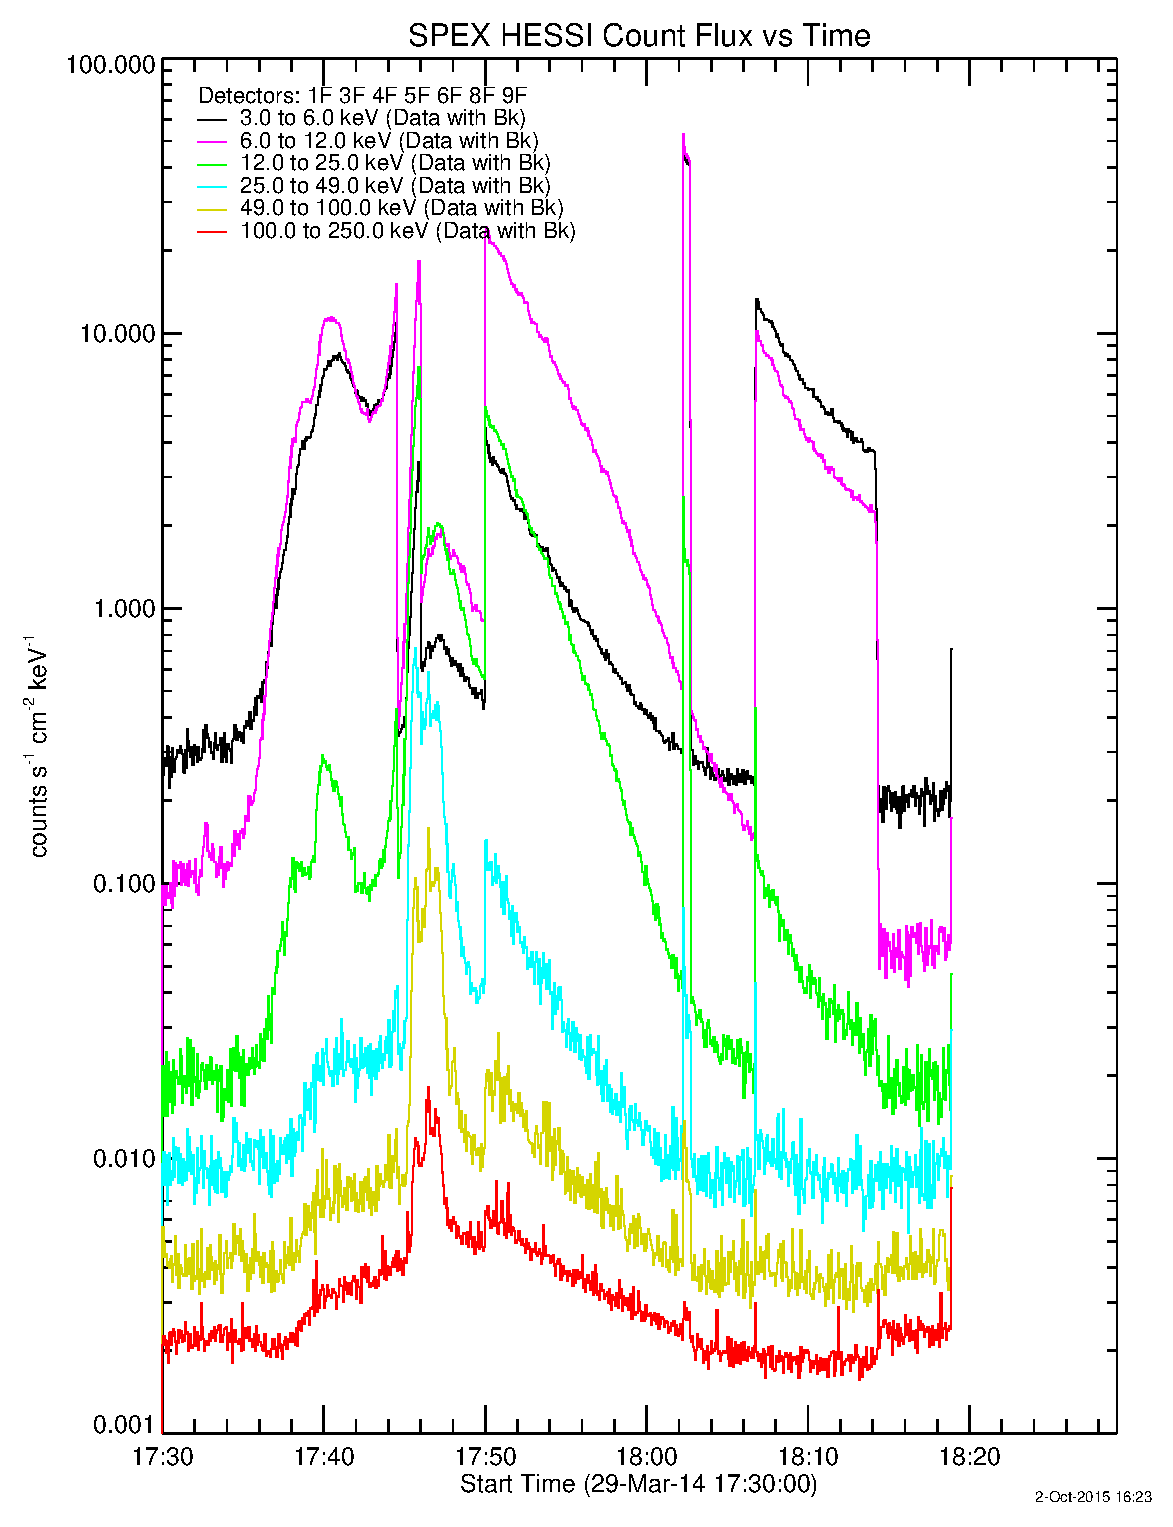
\includegraphics[width=0.7\textwidth]{count-flux-v-time-crop}
  \end{center}
  \caption{Shows RHESSI counts per area for multiple energy ranges. 3 to 6 keV in black, 6 to 12 keV in pink, 12 to 25 keV in green, 25 to 49 keV in turquoise, 49 to 100 keV in yellow and 100 to 250 keV in red. This range covers both thermal and non-thermal electron processes.}\label{rhessicft}
\end{figure}

The IRIS spacecraft captured the temporal evolution of the flare between 14:09 and 17:54 UT via it's slit-jaw imager and spectrograph instruments at solar coordinates of 491", 282" with a spatial resolution of 0.1667" per pixel. The slit-jaw imager data provides coverage of a field of view spanning 167" by 174", of passbands that including 1403, 2796 and 2832 \AA\ at 26, 19 and 75 second cadence respectively. The spectrograph slit is aligned directly over chromospheric flare ribbons, and the sunquake point of origin, with a field of view spanning 14" by 174". The spectrograph slit is exposed for $\sim9$ seconds at 8 slit locations for a total of 72 seconds cadence. Wavelengths observed over three channels include FUV1: 1331.7 - 1358.4 \AA, FUV2: 1389.0 - 1407.0 \AA\ and NUV: 2782.7 - 2851.1 \AA, associated with the upper-chromosphere down to the upper-photosphere. Spectral lines include C II, Si IV and Mg II h and k. IRIS data is the standard level 2 data product provided for scientific research, which has been calibrated to negate dark currents, flat-field and spacecraft rotational effects. The HMI instrument onboard SDO observed the entire solar photosphere, collecting 6173 \AA\ continuum intensity data throughout the flare event. HMI has a pixel size of 0.6 " providing reasonable spatial resolution at a cadence of 45 seconds. HMI data is calibrated to negate cosmic-rays, dark currents, flat-field and spacecraft rotational effects. A 6mHZ acoustic egression power map revealing the location of the sunquake is generated via holography techniques (supplied via private communication by Sergei Zharkov). HXR data from RHESSI and acoustic power data are overlaid on HMI and IRIS slit jaw maps for context, see Figure \ref{saxcontours-vert}.\\

\begin{figure}[H]
  \begin{center}
  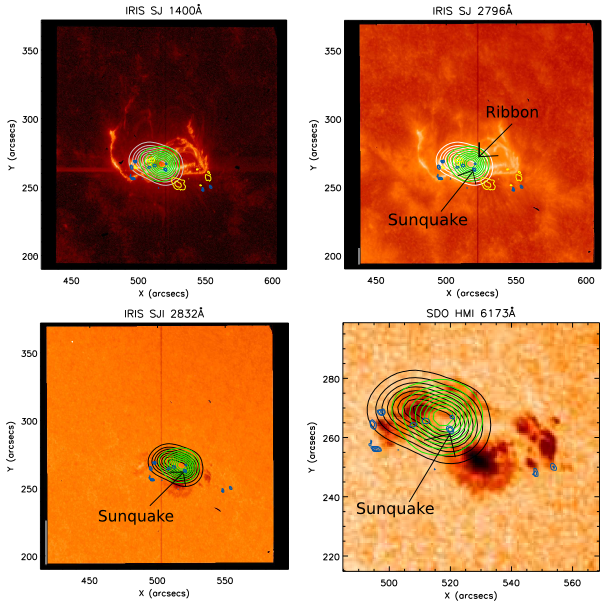
\includegraphics[width=1.0\textwidth]{saxcontours-square}
  \end{center}
  \caption{From top left to bottom right, images represent regions of the solar atmosphere at descending altitudes. The top two and bottom left images show IRIS SJ intensity maps of $1403$\AA\ (transition Region), $2796$\AA\ (chromosphere) and $2832$\AA\ (upper-photosphere) data. The bottom right image is SDO HMI $6173$\AA\ continuum intensity from the photosphere. Contours show RHESSI HXR with $E = 25-50$ keV in white or black and HXR with $E = 50-100 keV$ in green, sunspot locations in yellow taken from HMI and 6mHz acoustic power in blue.}\label{saxcontours-vert}
\end{figure}


\subsection{Analysis}

During the impulsive phase of a flare, high energy emission is an indicator that accelerated particles are present. Assuming that the chromosphere is a thick target \citep{1971SoPh...18..489B}, then the deposition of energy by accelerated particles will be by collisions between charged particles and ions producing hard X-ray bremsstrahlung emission.
 
\begin{equation}\label{pnth}
P(E \geq E_{c}) = \int_{E_{C}}^{\infty} EF(E)dE
\end{equation}

The thick target model allows for the integration of the total non-thermal electron power $P$ via equation \ref{pnth}. The electron distribution $F(E)$ is controlled by the power law $AE^{-\delta}$, where $E$ is the electron energy, $A$ is the total injected electron rate normalisation factor, $E_{C}$ is the low energy cut off and $\delta$ is the electron distribution spectral index.   
Performing the integral gives the total non-thermal electron power in the form of equation \ref{pnth1} .

\begin{equation}\label{pnth1}
P(E \geq E_{c}) = \frac{AE_{C}^{(2-\delta)}}{(\delta - 2)}
\end{equation}

The value of $E_{C}$ represents the upper boundary between thermal and non-thermal energy contributions to the x-ray spectrum. This means that the total energy associated with non-thermal electron power calculated by equation \ref{pnth1} is a lower limit.
  
Using the \texttt{ospex} software within SolarSoft (SSWIDL) RHESSI data are fit using the thick target non-thermal electron model. The entire data set has to be split into short intervals to improve the accuracy of fitting and the detail of resulting plots. Also the attenuator state of the instrument has to be taken into account due to differences in sensitivity to incoming photons. Therefore it is important to define intervals for fitting first by the attenuator state as \texttt{ospex} will mitigate for the differences in count sensitivity. Shown in Figure \ref{erhessi} is the resulting fit over the majority of the impulsive phase of the flare. At the peak of the impulsive phase between 17:46 and 17:47 the RHESSI fit shows an energy ranging from $1.0{\times}10^{28}$ to $2.5{\times}10^{29}$ erg. Assuming the fitting model is correct then the release of this energy is due to non-thermal electrons being accelerated and depositing energy into the chromosphere. 

\begin{figure}[H]
  \begin{center}
  \textbf{RHESSI 10 - 100 keV Hard Xray Energy Over Time}\par\medskip
  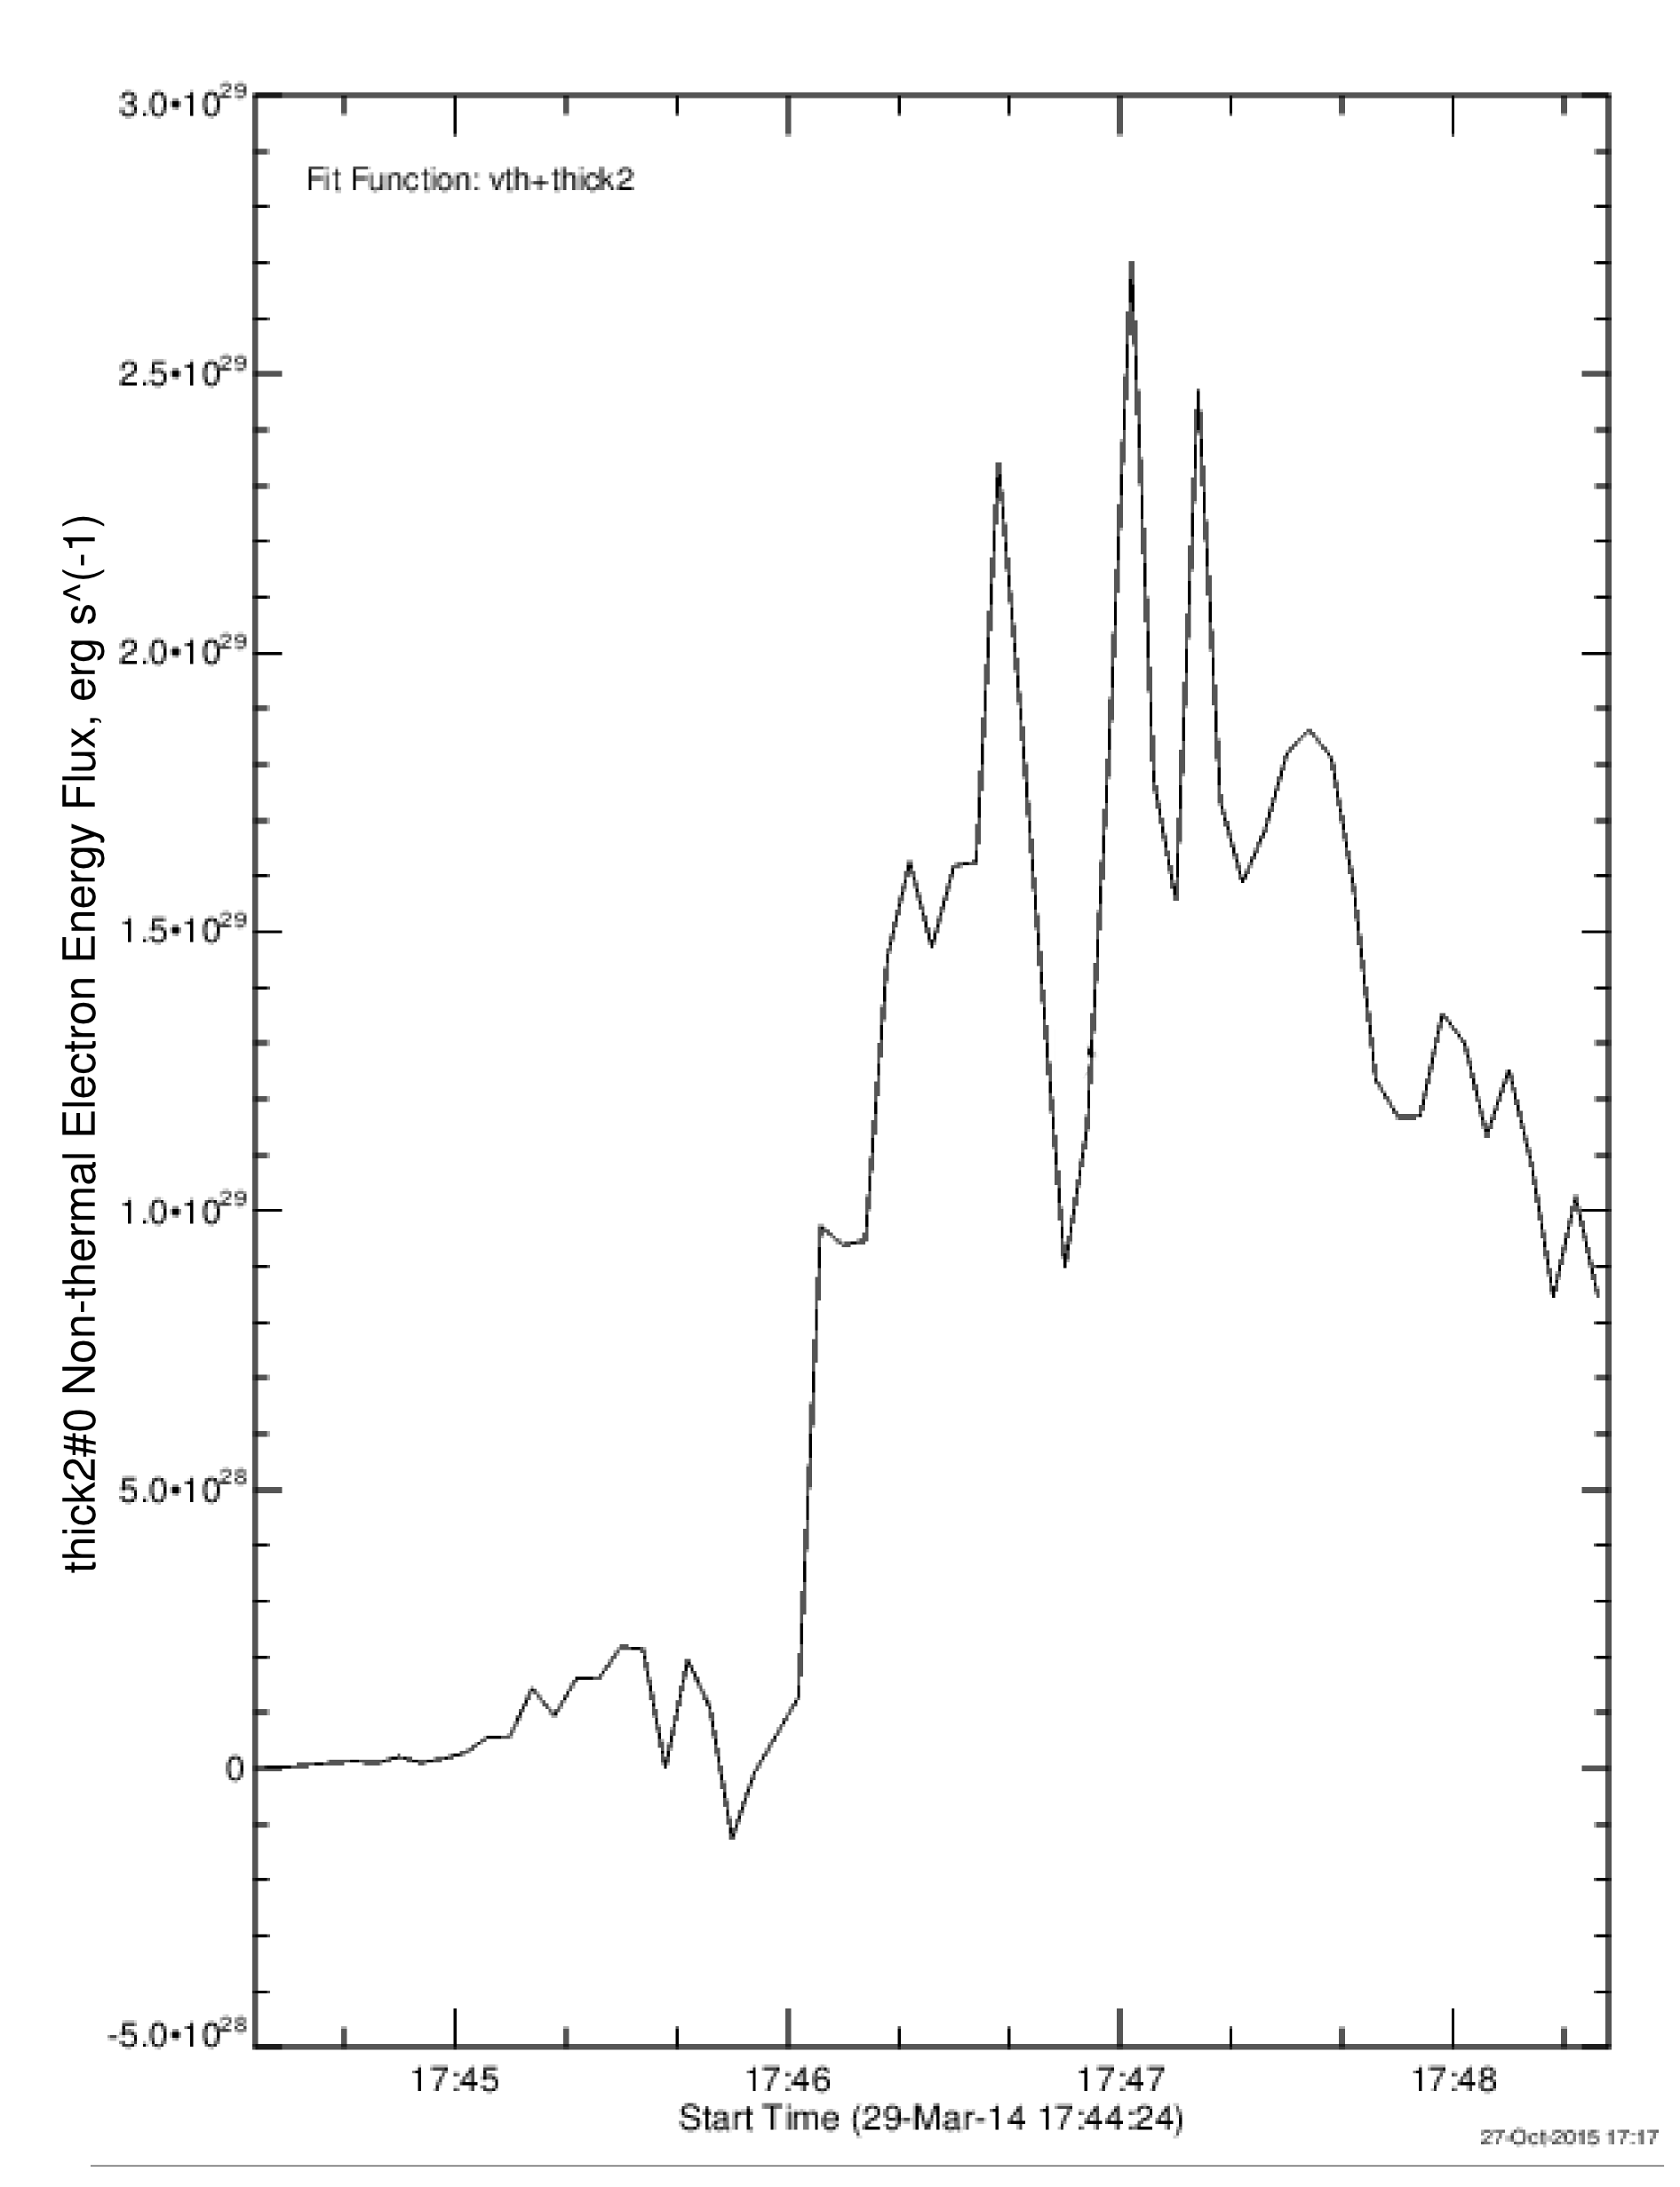
\includegraphics[width=0.6\textwidth]{rhessi-energy-curve}
  \end{center}
  \caption{Shows the energy evolution of hard x-ray emission collected by RHESSI 10 to 100 keV bins. Energy units are calculated by fitting a non-thermal electron model to the data. }\label{erhessi}
\end{figure}

White light flares are difficult to see against the bright photospheric background therefore to maximise the insight gained from observations of the flaring photosphere, data must be filtered. Silimarly to \cite{2014ApJ...783...98K}, photospheric data captured by IRIS MG II wing slit-jaw and SDO HMI continuum observations are subjected to a running difference filter to isolate locations that are white-light enhanced. The running difference filter effectively removes static features leaving behind those pixels that are changing over short time-scales. However, for removing signatures of those processes occurring over shorter time periods such as granulation and p-mode oscillations, this filtering technique is ineffective. This is not a problem, as for the purpose of white light flare analysis, the data yield a strong contrast between flare-enhanced and background pixels after being filtered by a $i-2$ running difference. The next stage is to determine which pixels in the difference image are those that are enhanced during the flare. For the best result, white-light enhanced pixels are identified using a combination of visual inspection and thresholding. Attempts at automating the identification process tend to lead to false positives being triggered by noise or granulation features. IRIS SJIs and SG data have no need for filtering.

%insert figure showing unfiltered and filtered iris and hmi data. 2x3: 2 unfiltered at the top, 2 filtered at the bottom, 2 thresholded showing only flare pixels.
%\graphicspath{ {~/PhD/Thesis/upgrade-plots/} }
\begin{figure}[H]
  \begin{center}
  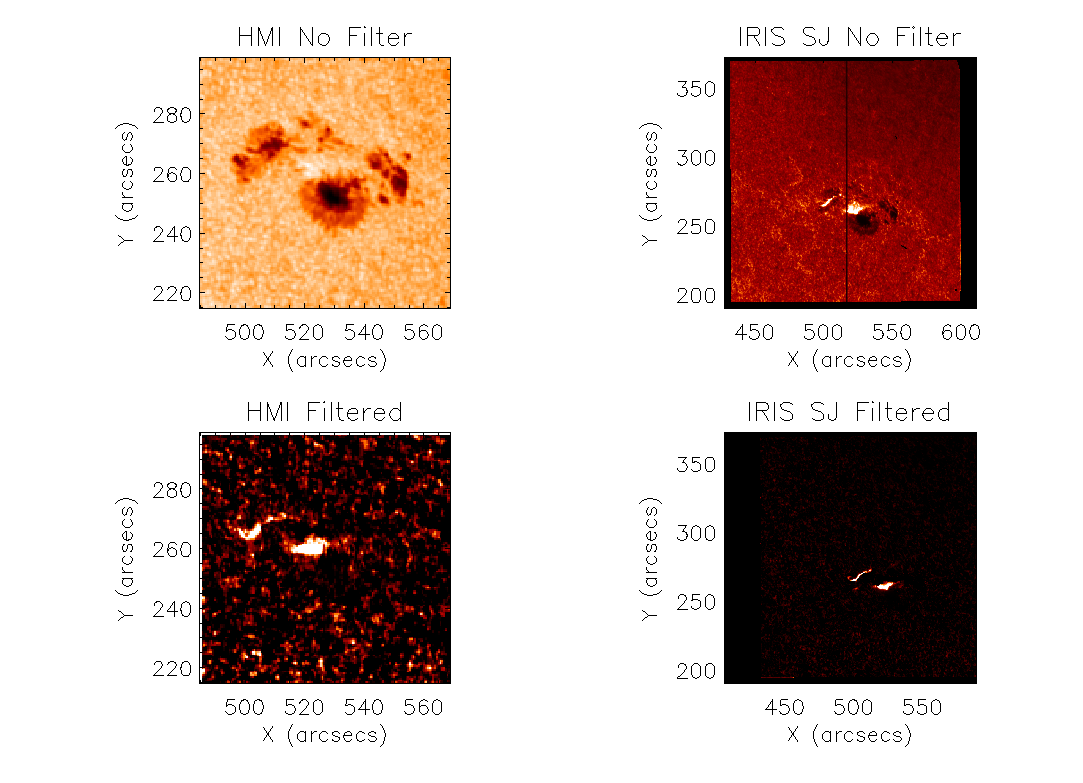
\includegraphics[width=0.8\textwidth]{29-Mar-14-diff-examples}
  \end{center}
  \caption{White light flares are difficult to observe against the bright photosphere requiring processing with a running difference filter to enhance ribbon features. The figure shows IRIS SJ 2832 \AA\ and SDO HMI continuum data before (top) and after (bottom) filtering.}\label{dif_filter}
\end{figure}

IRIS SJ and SG data are converted from relative intensity (DN per pixel) to energy (erg) units using conversion factors. Provided in the instrument documentation \citep{2014SoPh..289.2733D} is a method for acquiring the conversion factors in SSWIDL. It is then a case of inserting IRIS DN per pixel intensity values into the equation \ref{irisradiometriccal}. $F_{DN}$ is flux in units of DN per pixel, $C_{d2p}$ is the DN to photon conversion factor, $E_{\lambda}$ is the photon energy and $E_{erg}$ is to put the result into erg units.  

\begin{equation}\label{irisradiometriccal}
E = \frac{F_{DN}  C_{d2p} E_{\lambda}}{E_{erg}}
\end{equation}

To perform the same conversion for SDO HMI data required a slightly different approach due to the non-existent DN to photon conversion factor. Using a combination of sources \citep{2012SoPh..275...41B, 2012SoPh..275..285C} the instrument's properties are used to fulfil a conversion factor in the form of equation \ref{hmiradiometriccal}. Where $g$ is the instrument gain, $QE$ is the quantum efficiency of the charged couple device and $A_{ap}$ is the instrument aperture area, all other terms hold the same meaning as in equation \ref{irisradiometriccal}.

\begin{equation}\label{hmiradiometriccal}
E = \frac{F_{DN} E_{\lambda}}{g QE A_{ap} E_{erg}}
\end{equation}


For the IRIS and SDO HMI data sets, multiple sample points have been chosen based on locations specific to the sunquake and ribbon activity. Figures \ref{sirib}, \ref{mgrib}, \ref{mgwrib} and \ref{hmirib} show the ribbon coordinates sampled from each data set. Studying the flare in this way allows the energy distribution along the ribbon to be analysed and provides a point of comparison for the sunquake location. Each data set has five sample points per ribbon, a procedure which is repeated at two time frames, 17:45 and 17:46, providing twenty individual energy measurements per data set. The number of sample points will likely be increased in the future to provide better spatial resolution for ribbon energy distribution analysis. The problem with defining multiple ribbon samples over five different data sets comes when one considers the morphology of the local magnetic field. Accelerated charged material can only travel along the magnetic field, so the shape of those field lines will dictate the location of emission therefore the morphology of the ribbon. With this in mind the sample of coordinates chosen is based on matching common morphological features seen in each data set.

%insert figures showing ribbon coords oplot
\begin{figure}[H]
  \begin{center}
  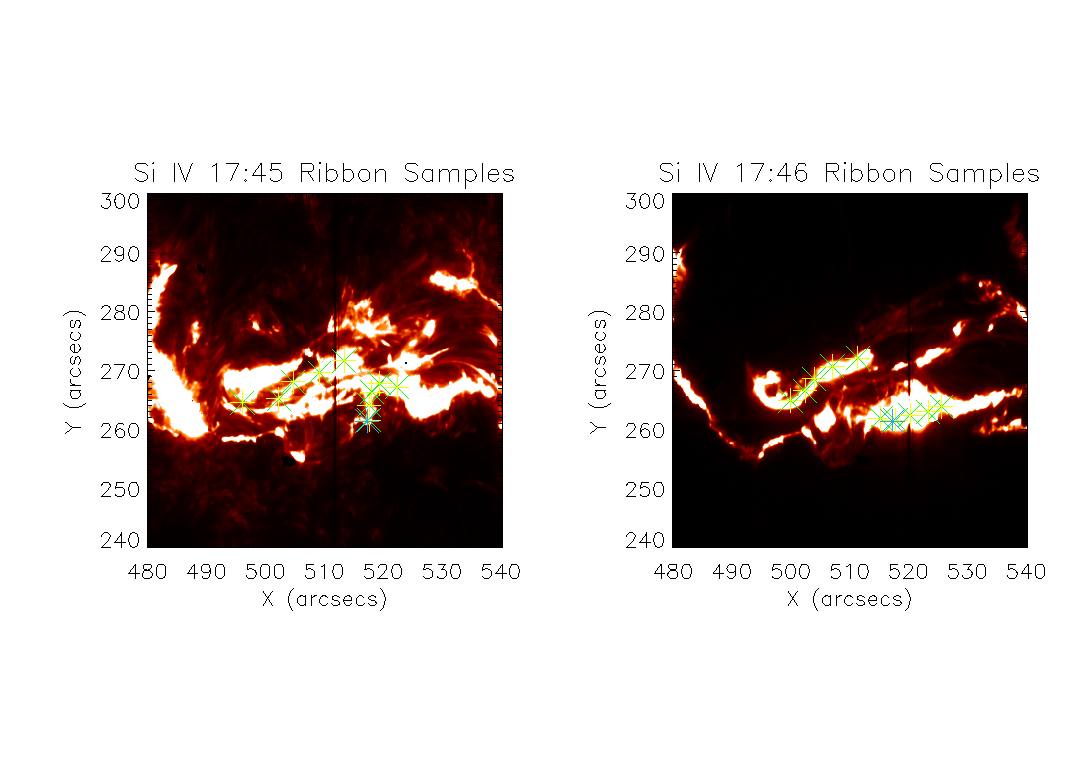
\includegraphics[width=0.8\textwidth]{29-Mar-14-SI-Ribbon-Coord-oplot}
  \end{center}
  \caption{Shows IRIS Si IV slit-jaw data with sampled ribbon and sunquake pixel coordinates marked in green and blue respectively. Twenty ribbon sample points are taken from two instances in time.}\label{sirib}
\end{figure}

\begin{figure}[H]
  \begin{center}
  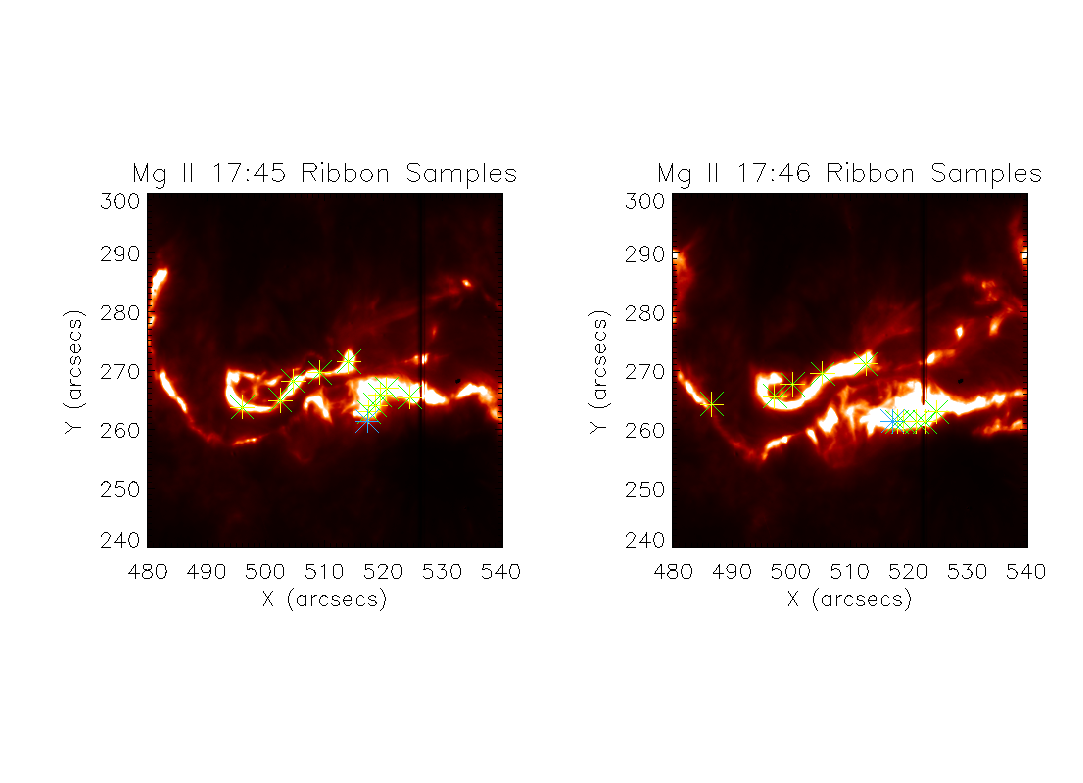
\includegraphics[width=0.8\textwidth]{29-Mar-14-MG-Ribbon-Coord-oplot}
  \end{center}
  \caption{Shows IRIS Mg II slit-jaw data with sampled ribbon and sunquake pixel coordinates marked in green and blue respectively. Twenty ribbon sample points are taken from two instances in time.}\label{mgrib}
\end{figure}

\begin{figure}[H]
  \begin{center}
  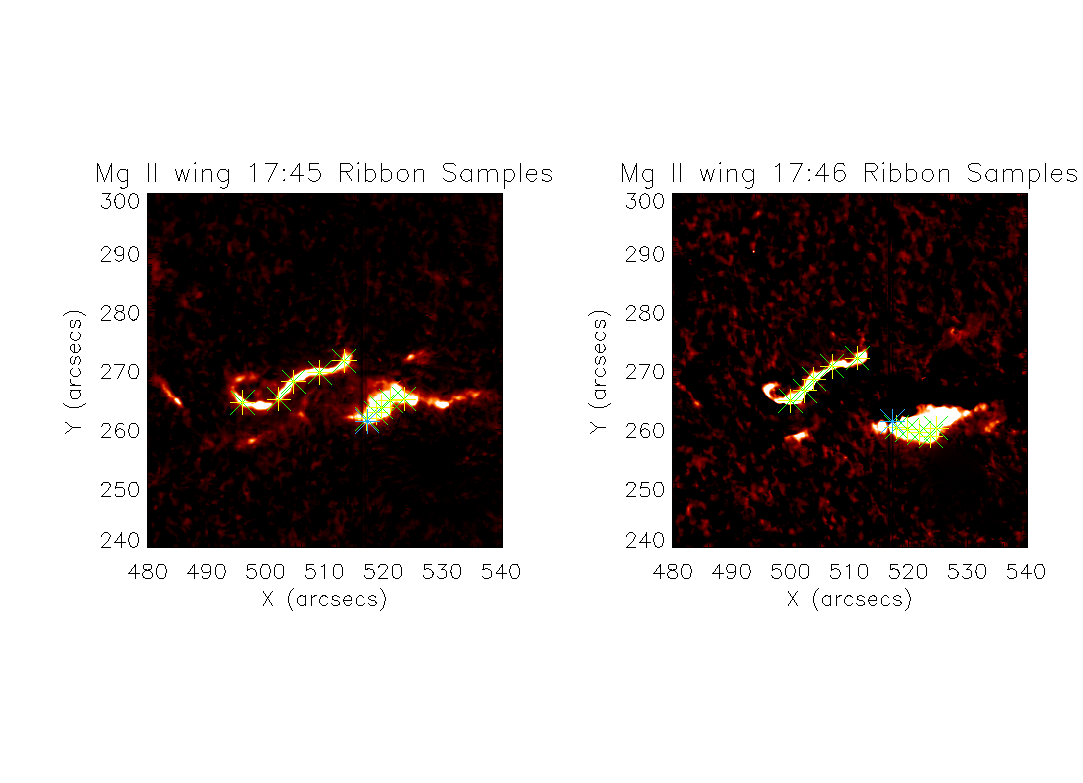
\includegraphics[width=0.8\textwidth]{29-Mar-14-MGW-Ribbon-Coord-oplot}
  \end{center}
  \caption{Shows IRIS Mg II wing slit-jaw data with sampled ribbon and sunquake pixel coordinates marked in green and blue respectively. Twenty ribbon sample points are taken from two instances in time.}\label{mgwrib}
\end{figure}

\begin{figure}[H]
  \begin{center}
  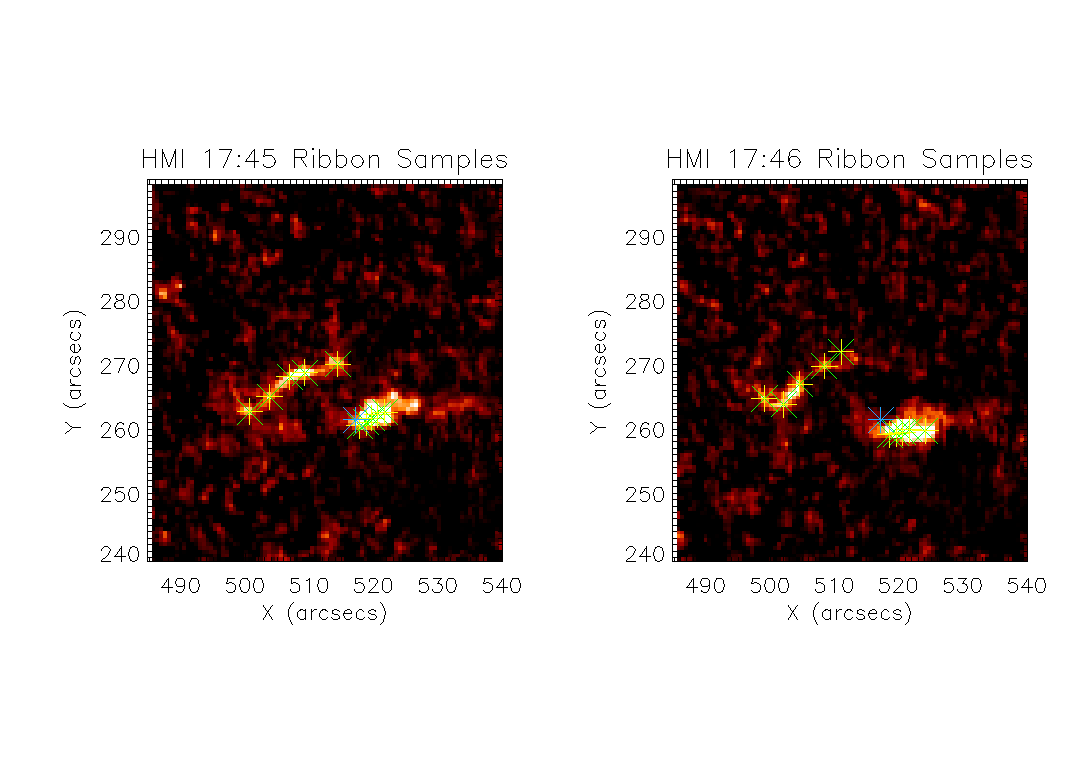
\includegraphics[width=0.8\textwidth]{29-Mar-14-HMI-Ribbon-Coord-oplot}
  \end{center}
  \caption{Shows SDO HMI continuum with sampled ribbon and sunquake pixel coordinates marked in green and blue respectively. Twenty ribbon sample points are taken from two instances in time. This procedure is also applied to IRIS SJ and SG data, see the Appendix for more figures.}\label{hmirib}
\end{figure}


IRIS spectroscopic data is sampled over a wavelength range of 2825.7 and 2825.8\AA\ (see \ref{balmercontinuum}) which is within the Balmer continuum. Balmer Data is sampled at slit positions and pixels that relate to one quake position and twenty ribbon samples, as with the other data sets. 

%insert figure showing balmer continuum spectrum sample range
\begin{figure}[H]
  \begin{center}
  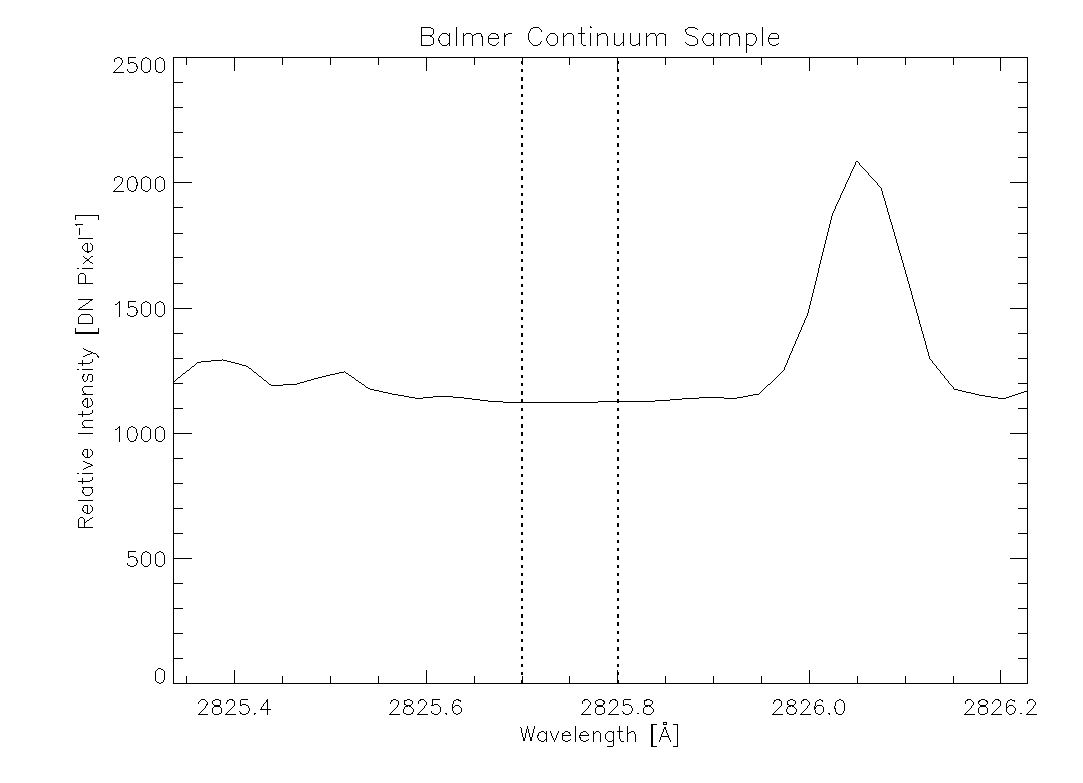
\includegraphics[width=0.8\textwidth]{29-Mar-14-Balmer-Continuum}
  \end{center}
  \caption{Shows the Balmer continuum component sampled from the IRIS SG data. Balmer emission is an indicator of radiative backwarming of the photosphere. }\label{balmercontinuum}
\end{figure}


Once all energies are calculated for each location and data set, time series energy-curves are created, see Figures \ref{erhessi} and \ref{eqk} (the Appendix contains the energy curves taken from ribbon locations). Each energy-time ladder plot contains energy curves from IRIS SJ 1400 \AA\, 2796 \AA\, SG Balmer, SJ 2832 \AA\ and SDO HMI continuum aligned in time. From top to bottom, the order of the plots in the ladder represents descending plasma temperature in the solar atmosphere see Tables \ref{iris-sg} and \ref{iris-sj}. Tables \ref{qkenergytab} and \ref{ribenergytab} display energy values taken from each pixel location and data set, except RHESSI, at two times corresponding to maximum WLF ribbon intensity at 17:45 and 17:46. Figure \ref{eqk} contains plots for the sunquake epicentre pixel, peak energies from each data set range from $9.63{\times}10^{14}$ erg from IRIS 1400 \AA\, $4.36{\times}10^{16}$ erg from IRIS 2796 \AA\ which is a lower limit due to over saturation of the instrument CCD, $2.68{\times}10^{16}$ erg from IRIS Balmer, $8.21{\times}10^{15}$ erg from IRIS 2832 \AA\ and $3.29{\times}10^{13}$ erg from SDO HMI continuum. 

\begin{figure}[H]
  \begin{center}
  \textbf{Quake Location Energy Over Time}\par\medskip
  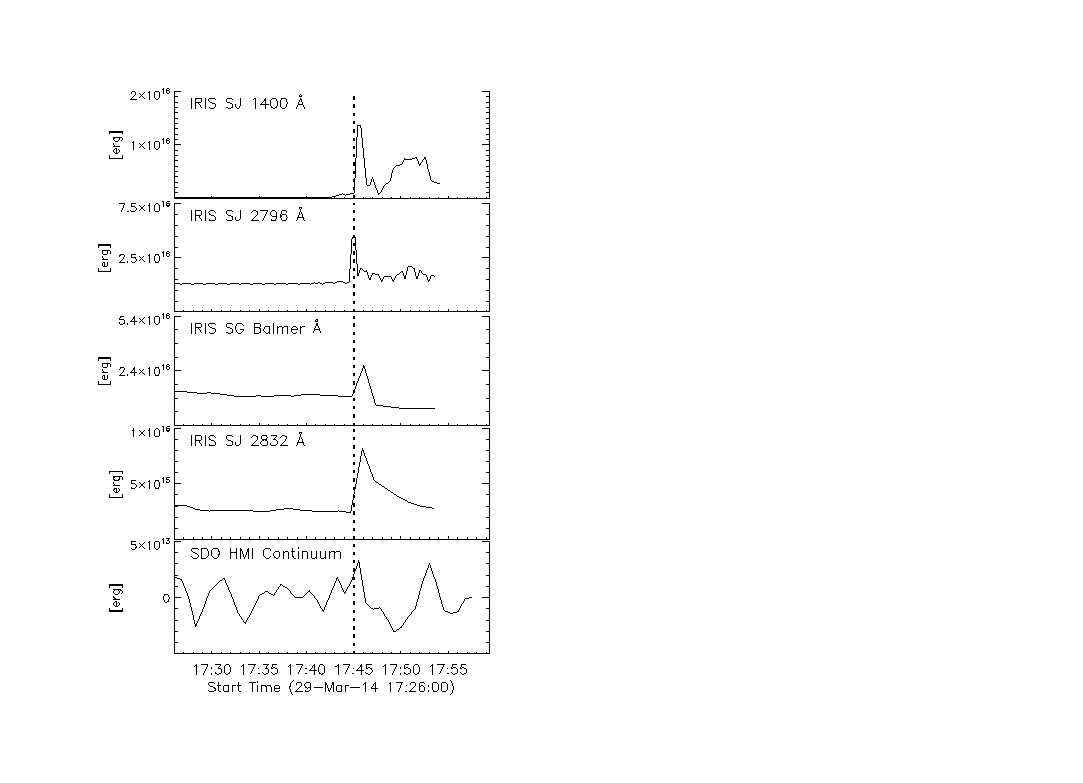
\includegraphics[width=0.6\textwidth]{29-Mar-14-Quake-Energy-Ladder}
  \end{center}
  \caption{Shows calculated energy values over time of the region thought to be the sunquake epicentre (518.5", 264.0"). Each plot represents an independent data set, in order from top to bottom the sets are; IRIS SJ 1400 \AA\ (Si IV); IRIS SJ 2796 \AA\ (Mg II); IRIS SG  2825.7 to 2825.8 \AA\ (Balmer Continuum);IRIS SJ 2832 \AA\ (Mg II wing); SDO HMI continuum (HMI). The dotted line running vertically through each plot signifies a the onset time of the eruptive phase of the flare}\label{eqk}
\end{figure}

Ribbon plots show a wide range of properties. In an order dictated by Table \ref{ribenergytab}. The following is a bulletized summary of each ribbon position ladder-plot. The ribbon location is based on the HMI coordinates.


Another consideration is that Figure \ref{eqk} only relates to one pixel, therefore to analyse the energy emitted from an area comparable to the sunquake origin area would provide a better estimate of the radiative energy available. This has been calculated for HMI continuum data only, based on the sunquake area $2.6{\times}10^{16}$ $cm^{2}$ as stated in \cite{2014ApJ...796...85J}. Based on this area value 13 HMI pixels are sampled, summed and converted to energy, producing an upper limit of $2.54{\times}10^{17}$ erg. Comparing this to the sunquake energy, $1.3\pm0.05{\times}10^{26}$ $erg.s^{-1}$, also stated in \cite{2014ApJ...796...85J} to the hmi area estimate shows that the sunquake contains $10^{9}$ times more energy. 





\subsection{Results and Discussion}

This project presents a first look at a multi-wavelength energy analysis of the lower solar atmosphere during the 29th of March 2014 X class solar flare. The main focus up to this point has been to acquire energy estimates from the various atmospheric regions in an attempt to assess the likelihood of radiative backwarming as a generation method for the sunquake. The location of maximum acoustic power, RHESSI HXR, IRIS and SDO intensity correlate both spatially and temporally (see Figure \ref{saxcontours-vert}), showing that energy input into the upper chromosphere via accelerated non-thermal electrons propagates down to the photosphere. The sunquake is located directly underneath both maximum HXR and an area of white-light emission.

Energy estimates from RHESSI data show there to be between $1.0{\times}10^{28}$ to $2.5{\times}10^{29}$ erg during the impulsive phase of the flare. Comparing this to the sunquake energy of $1.3\pm0.05{\times}10^{26}$ $erg.s^{-1}$ means that the acoustic energy is well within the energy budget provided by accelerated non-thermal electrons, so how is the energy getting to the photosphere to cause seismic event?

Energy estimates from IRIS are not always useful due to over saturation of the instrument CCD, however, when comparing the ribbon locations to that of the sunquake some clear behaviours reveal themselves. The 1400 \AA\ channel is almost always showing greater radiative energy in all ribbon locations compared to the sunquake. This could be because transition region ribbons are rarely directly above the sunquake epicentre due to magnetic field configuration. The 2796 \AA\ channel becomes saturated slightly less often than the 1400 \AA\, providing more insight. The IRIS 2796 \AA\ channel is less in energy than the sunquake location around 30\% of the time. However, no real comparison can be attained due to the saturation of the CCD at the majority of ribbon pixels and the sunquake pixel. The only information that can be deduced, is that the sunquake pixel has an extraordinary 2796 \AA\ enhancement but then so do the majority of the ribbon locations. Balmer emission calculated from IRIS SG data is consistently of less energy than at the sunquake location, this is an interesting result as it means that there is more radiative backwarming above the sunquake pixel than in any other location sampled. However, the energy required to generate the sunquake is in the order of $10^25$ ergs, which when compared to the $2.68{\times}10^{16}$ erg of energy available in the Balmer pixel is $10^{9}$ times greater! Perhaps radiative backwarming only plays a bit-part in the generation of the sunquake?  
The 2832 \AA\ IRIS channel is harder to summarise due to the fact that comparing ribbon locations to that of the sunquake show that there is a 50:50 chance that the ribbon could have greater or lower energy output.
SDO HMI continuum data is probably the most revealing, in that almost all of the ribbon locations have far greater energy output than the sunquake location. This could be explained by the sunquake being only partially under a white light ribbon. 

In conclusion, this analysis has barely scratched the surface of the information available in the data. Some immediate trends have been noticed such as the lower levels of Balmer and higher levels of photospheric continuum energy in the flare ribbons compared to the sunquake. Is there a connection between these two emission regions, and do these signatures have anything to do with the generation of the sunquake? In general the data sets available are tending to show that there is not enough energy in atmospheric emission to generate the sunquake via radiative backwarming.

  

\subsection{Future Work}
Obviously there is a need for a much more detailed analysis, which will be the main task for the immediate future. Plotting energy behaviours of each ribbon location and data set would help to visualise the trends discussed. There is plans to analyse $\gamma$-ray and magnetogram data to look for signatures associated with direct particle collision and impulsive magnetic field reconfiguration respectively. IRIS SG data will be used to analyse Doppler-shift to look for shock waves.

\subsubsection{In the Last Few Months}
The majority of the work carried out since the last panel meeting has been:
\begin{itemize}
\item Calculate energy associated with emission captured by HMI to compare with the acoustic power of the sunquake.
\item Calculate energy associated with emission captured by IRIS slit jaw and spectrometer in order to estimate energy deposition in the atmosphere.
\item Calculate energy associated with Balmer emission to assess likely energy contribution of radiative backwarming.
\item Calculate non-thermal electron power via HXR spectra to estimate the initial energy of the electron beam accelerated by the corona.
\end{itemize}



